% ---
% Capitulo de revisão de literatura
% ---

\chapter{Análise da Rede}

\section{Sumarização de indicadores descritivos}

De imediato, é possível aferir alguns dados básicos da rede completa com o auxílio do \textit{Networkx} ou do \textit{Gephi}:

\begin{itemize}
	\item Número de nós: 32.881 (maior do que o número de registros pois cada registro contém um elenco com N atores/atrizes)
	\item Número de arestas: 252.055
	\item Grau médio:  15,33 (média de ligações/interações de cada vértice/ator)
\end{itemize}

Conforme descrito na modelagem da rede, optou-se pro obter o sub-grafo da componente gigante da rede, cuja cobertura inclui cerca de 89,5\% dos vértices da rede:

\begin{itemize}
	\item Número de vértices: 29.440
	\item Número de arestas: 241.744
	\item Grau médio:  16,42
	\item Densidade: 0,000557 (Razão entre número de arestas existentes/possíveis)
	\item Diâmetro: 17 (caminho mais longo possível entre quaisquer 2 vértices da rede)
	\item Coeficiente de \textit{clustering} médio: 0,824 (Alta probabilidade devido às “aglomerações locais” do \textit{elenco} de cada registro, onde todos os nós têm ligações entre si)
	\item Comprimento médio de caminho: 5,647 (Distância média, em númeo de vértices, que deveria ser percorrida para alcance entre dois vértices arbitrários)
	\item Fechamento triadíco: 0,39849 (Probabilidade de formação de “triângulos” - relativamente alta pelo mesmo motivo do coeficiente de \textit{clustering})

\end{itemize}

A figura \ref{fig:grau-netflix} auxilia na visualização de como os graus dos vértices da rede estão distribuídos. A distribuição é exibida de forma que o eixo X representa a cardinalidade possível do grau do vértice de acordo com as ocorrências na base, enquanto no eixo Y está representado sua probabilidade, de acordo com o número efetivo de ocorrências. O grau 9 (ou seja, o ator/atriz co-atuar com 9 outros atores), por exemplo, de maior ocorrência, tem uma probabilidade um pouco maior que 16\%.

\begin{figure}[!htb]
\centering
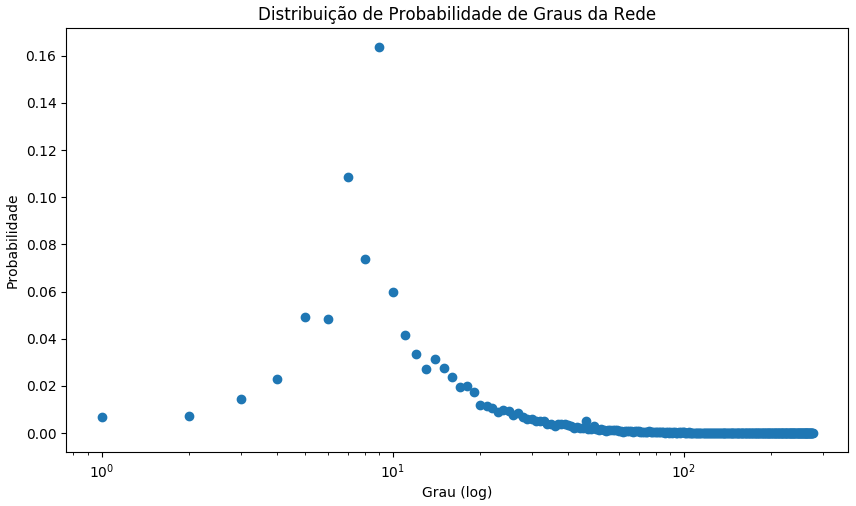
\includegraphics[width=13cm]{img/grau-probabilidade-netflix.png}
\caption{Distribuição de graus da rede x probabilidade de ocorrência}
\label{fig:grau-netflix}
\end{figure}


\section{Detecção de comunidades}

Para detecção de comunidades na rede, foram utilizados os algoritmos de modularidade e método de Louvain (que consiste em um aprimoramento do método anterior) respectivamente no Networkx e no Gephi. Pelo método de Louvain, foram obtidas 93 comunidades, contendo a maior delas 4.823 vértices, a menor 5 vértices, e uma média de 313,19 vértices por comunidade. No Gephi, o método de modularidade gerou 99 comunidades.

\begin{figure}[!htb]
\centering
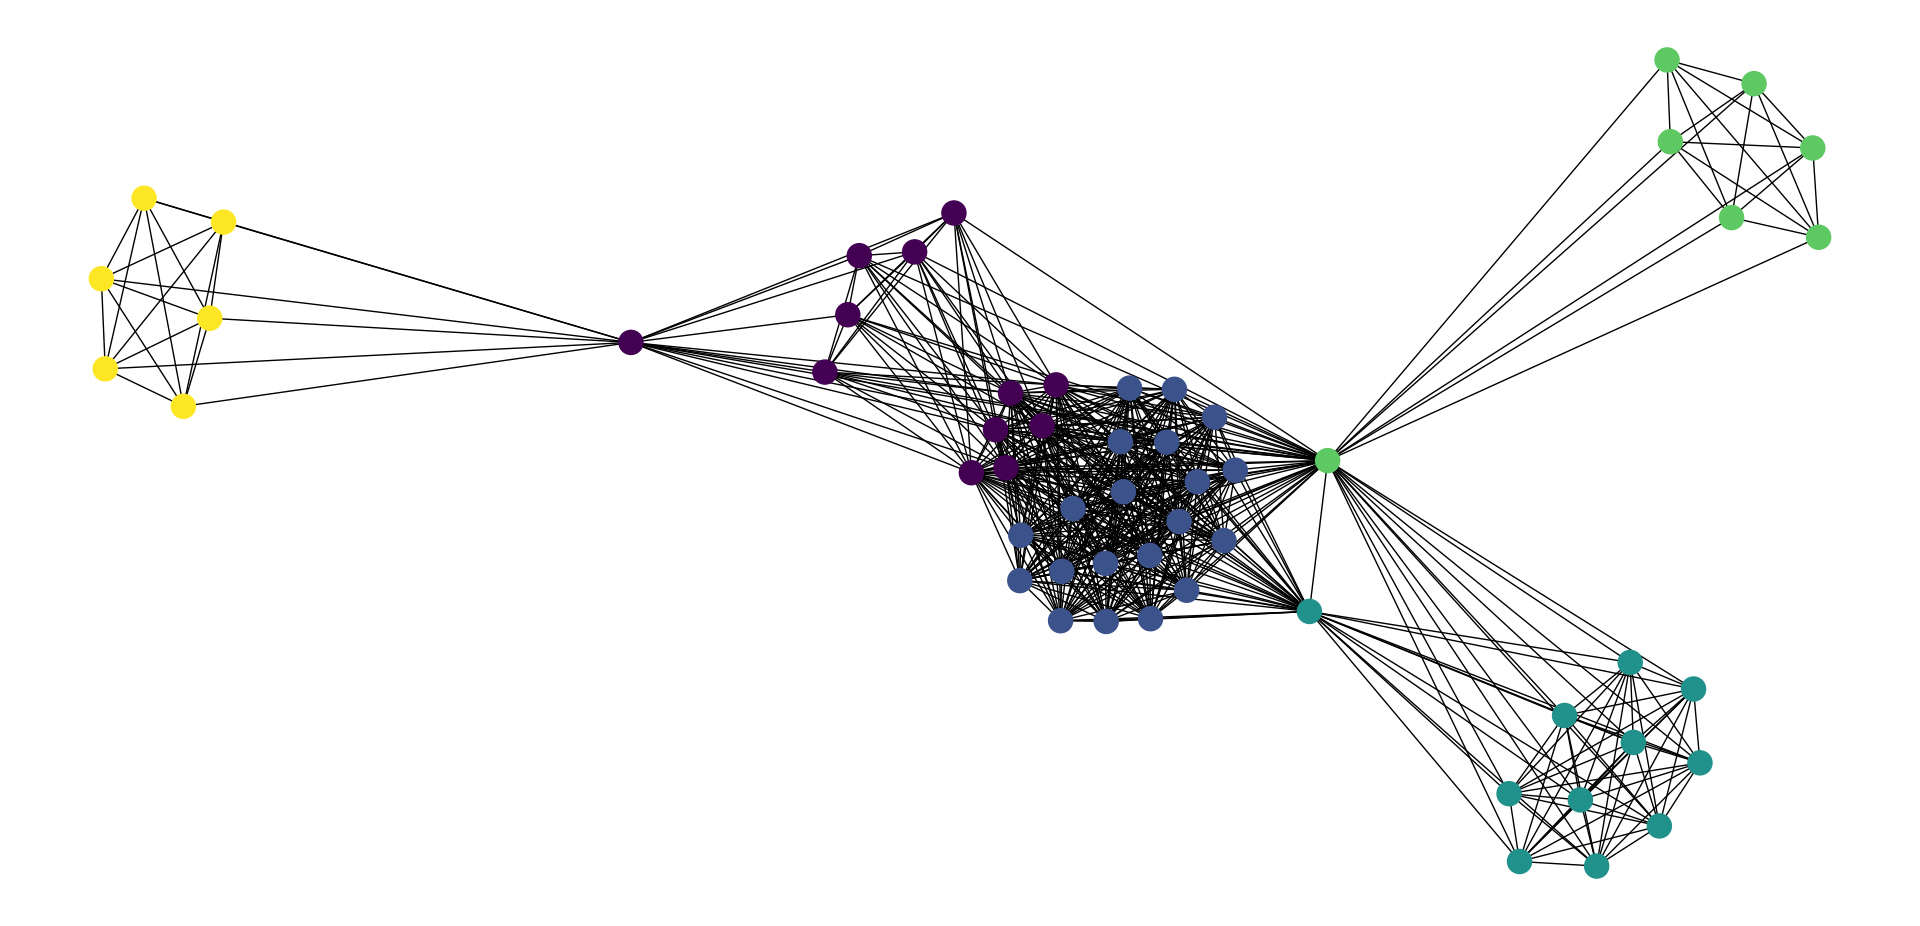
\includegraphics[width=14cm]{img/Figure_3.png}
\caption{Divisão de comunidades no NetworkX - Método de Louvain}
\label{fig:sub-comunidades}
\end{figure}

A figura \ref{fig:sub-comunidades} ilustra, para uma amostra pequena, uma ideia da divisão de comunidades no NetworkX. Pela característic ada modelagem da rede, espera-se esse comportamento onde hajam vários pequenos grupos conectados (correspondentes aos elencos individualmente) e alguns vértices como é possível observar na imagem que fazem essas pontes dentre os aglomerados. Em uma visão geral, devido ao grande número de vértices e arestas, se torna difícil fazer qualquer inferência ou dar algum significado, como mostra a figura \ref{fig:grafo_overview}, gerada com o método de modularidade do Gephi, atribuindo cores diferentes para cada comunidade.

\begin{figure}[!htb]
\centering
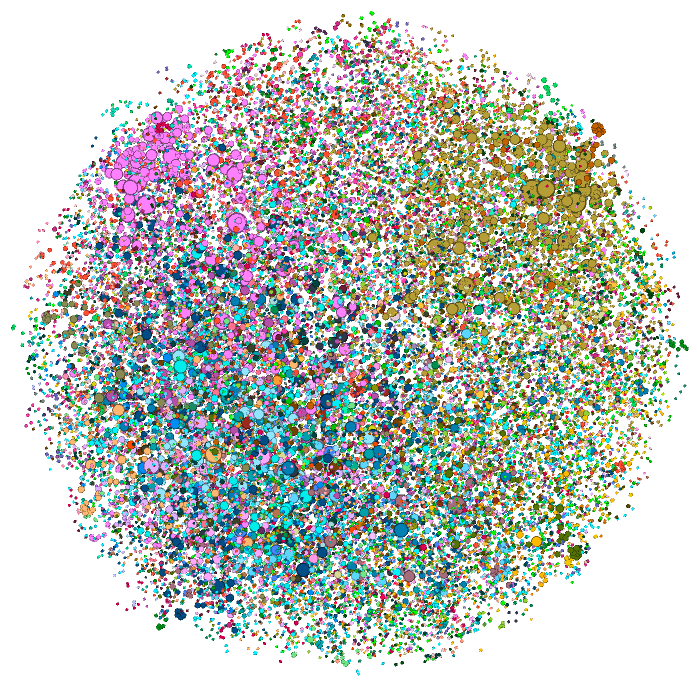
\includegraphics[width=12cm]{img/grafo_overview.png}
\caption{Visão geral das comunidades utilizando partição de modularidade no Gephi}
\label{fig:grafo_overview}
\end{figure}


\section{Rankeamento e centralidade vértices}

Do ponto de vista individual das entidades ou vértices da rede, com frequência é pertinente à aplicação estabelecer algum critério para classificar os vértices mais importantes. Essa importância denotada não é um conceito rígido e final, mas que flexivelmente depende do contexto da aplicação e passível de interpretação. Em cada cenário possível (estratégias de marketing, no estudo de disseminação de doenças, dentre outros exemplos) a escolha de uma métrica ou critério pode tomar uma conotação diferente. Para ilustrar essas possibilidades, 4 métricas são aplicadas para obter os vértices mais bem classificados segundo esses critérios.

O primeiro deles, o grau de entrada refere-se de forma direta ao número de conexões (ou, no contexto da base, quem co-atuou com mais atores diferentes). A centralidade de proximidade (\textit{closeness}) é uma forma de detectar nós que são capazes de espalhar informações de forma eficiente e mede sua distância média para todos os outros nós. A centralidade por intermediação (\textit{betweenness}) refere-se ao número de menores caminhos de todos os vértices para quaisquer outros vértices que passam por aquele nó. Por fim, a centralidade por auto-vetor é baseada na noção de que a influência de um vértice é dada não de forma individual, mas existe uma influência mútua, onde um vértice que faz interação com um vértice de maior influência, é potencialmente um vértice com maior influência (ideia base do algoritmo de \textit{pagerank}). A tabela \ref{tab:rankeamento vertices} apresenta os atores melhor classificados em cada critério, juntamente com o respectivo índice.

\begin{table}[h]
\footnotesize
\centering

\caption{Rankeamento e centralidade dos vértices} % igual ao ambiente figura
\begin{tabular}{|m{3.5cm}|m{3.5cm}|m{3.5cm}| m{3.5cm}|}

\hline
\multicolumn{1}{|c|}{\textbf{Maior Grau}} & \multicolumn{1}{c|}{\textbf{Betweenness}} & \multicolumn{1}{c|}{\textbf{Closeness}} & \multicolumn{1}{c|}{\textbf{Auto-vetor}} \\
\hline


Anupam Kher: 277 & Anupam Kher: 0.059 & Gerard Butler: 0.267
 & Takahiro Sakurai: 0.16\\
\hline

Shah Rukh Khan: 212 & Om Puri: 0.03 & Alfred Molina: 0.265 & Yuichi Nakamura: 0.15\\
\hline

Takahiro Sakurai: 208 & Sahajak Boonthanakit: 0.028 & Ben Kingsley: 0.264 & Yuki Kaji: 0.15\\
\hline

Yuki Kaji: 202 & Iko Uwais: 0.026 & Chloe Grace Moretz: 0.263 & Jun Fukuyama: 0.14\\
\hline

Fred Tatasciore: 197 & Ben Kingsley: 0.025 & Helen Mirren: 0.262 & Junichi Suwabe: 0.13\\
\hline

Yuichi Nakamura: 196 & Cesar Montano: 0.025 & James Franco: 0.262 & Katsuyuki Konishi: 0.13\\
\hline

Fred Armisen: 189 & Steven Yeun: 0.025 & Samuel L. Jackson: 0.261 & Kana Hanazawa: 0.12\\
\hline

Akshay Kumar: 188 & Kari Wahlgren: 0.022 & Jacki Weaver: 0.261 & Eri Kitamura: 0.12 \\
\hline

Om Puri: 187 & Haluk Bilginer: 0.021 & Lena Headey: 0.261 & Daisuke Ono:  0.12\\
\hline

Boman Irani: 183 & Christopher Lee: 0.021 & Willem Dafoe: 0.260 & Hiroshi Kamiya: 0.12\\

\hline
\end{tabular}
\label{tab:rankeamento vertices}
\end{table}



\section{Comparação com o processo de geração aleatório (Erdõs-Rényi)}

Para a etapa de inspeção e verificação com relação ao quanto a formação da rede se aproxima de um processo aleatório, gerou-se um modelo de Erdős–Rényi utilizando os parâmetros da componente principal para quantidade de nós e densidade. A rede obtida, como esperado, tem 29.440 nós e um número bem próximo de arestas (241.853, que anteriomente eram 241.744). O grafo gerado possui um único componente conectado, que por definição é também a componente gigante.

Os coeficientes de aglomeração/triangulação, por sua vez, são significativamente menores que a rede original (o que é esperado, já que não segue a definição do modelo que gera os cliques): 0.000587 e 0.000582, respectivamente. A diferença na formação das redes fica evidente ao observar a distribuição de graus dos nós na figura \ref{fig:comparacao}. Enquanto a rede em estudo segue uma lei de potência em sua distribuição (característica de redes do mundo real), a rede gerada aleatoriamente segue uma distribuição normal (característica de redes geradas aleatoriamente).


\begin{figure}[H]
	\centering
  	\subfigure[Rede em estudo (Netflix)]{
   	 	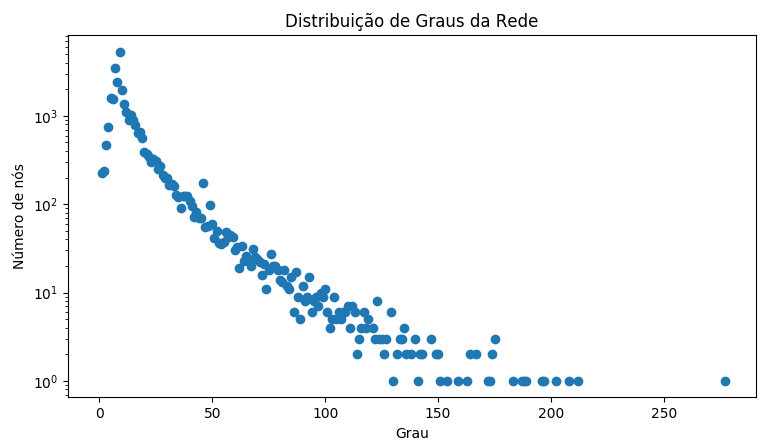
\includegraphics[width=12cm]{img/grau-netflix.png}
    		\label{subfig:grau-netflix}}
    		\hfill
  	\subfigure[Rede de Erdős–Rényi]{
    		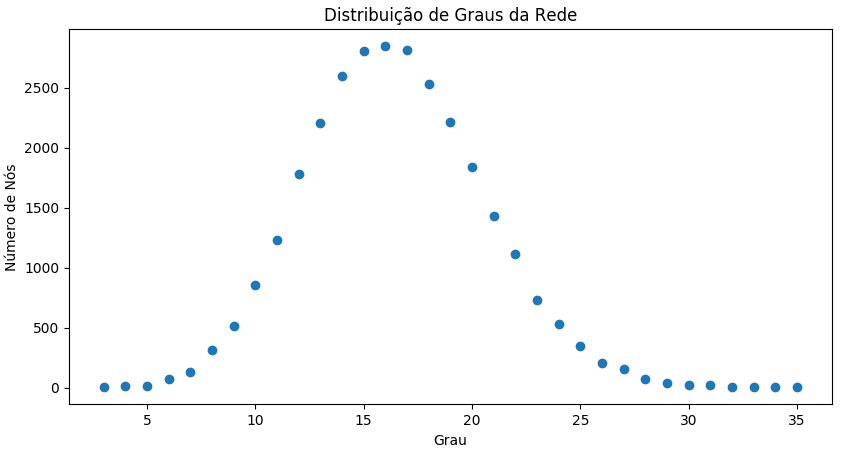
\includegraphics[width=12cm]{img/grau-erdos.png}
    		\label{subfig:grau-erdos}} 
  	\caption{Distribuição de graus}  
  	\label{fig:comparacao}
\end{figure}	
	
